% Copyright 2004 by Till Tantau <tantau@users.sourceforge.net>.
%
% In principle, this file can be redistributed and/or modified under
% the terms of the GNU Public License, version 2.
%
% However, this file is supposed to be a template to be modified
% for your own needs. For this reason, if you use this file as a
% template and not specifically distribute it as part of a another
% package/program, I grant the extra permission to freely copy and
% modify this file as you see fit and even to delete this copyright
% notice. 

\documentclass{beamer}
\usepackage[utf8]{inputenc}
\usepackage[brazilian]{babel}

% There are many different themes available for Beamer. A comprehensive
% list with examples is given here:
% http://deic.uab.es/~iblanes/beamer_gallery/index_by_theme.html
% You can uncomment the themes below if you would like to use a different
% one:
%\usetheme{AnnArbor}
%\usetheme{Antibes}
%\usetheme{Bergen}
%\usetheme{Berkeley}
%\usetheme{Berlin}
%\usetheme{Boadilla}
%\usetheme{boxes}
\usetheme{CambridgeUS}
%\usetheme{Copenhagen}
%\usetheme{Darmstadt}
%\usetheme{default}
%\usetheme{Frankfurt}
%\usetheme{Goettingen}
%\usetheme{Hannover}
%\usetheme{Ilmenau}
%\usetheme{JuanLesPins}
%\usetheme{Luebeck}
%\usetheme{Madrid}
%\usetheme{Malmoe}
%\usetheme{Marburg}
%\usetheme{Montpellier}
%\usetheme{PaloAlto}
%\usetheme{Pittsburgh}
%\usetheme{Rochester}
%\usetheme{Singapore}
%\usetheme{Szeged}
%\usetheme{Warsaw}

\title{Aula 1 - Unix}

% A subtitle is optional and this may be deleted
\subtitle{Curso de Unix}

\author{PET Computa\c{c}ão}
% - Give the names in the same order as the appear in the paper.
% - Use the \inst{?} command only if the authors have different
%   affiliation.

\institute[UFSC] % (optional, but mostly needed)
{
%
  Departamento de Informática e Estatística\\
  Universidade de Santa Catarina}
% - Use the \inst command only if there are several affiliations.
% - Keep it simple, no one is interested in your street address.

\date{PET Computa\c{c}ão, 2015}
% - Either use conference name or its abbreviation.
% - Not really informative to the audience, more for people (including
%   yourself) who are reading the slides online

\subject{Curso de Unix}
% This is only inserted into the PDF information catalog. Can be left
% out. 

% If you have a file called "university-logo-filename.xxx", where xxx
% is a graphic format that can be processed by latex or pdflatex,
% resp., then you can add a logo as follows:

% \pgfdeclareimage[height=0.5cm]{university-logo}{university-logo-filename}
% \logo{\pgfuseimage{university-logo}}

% Delete this, if you do not want the table of contents to pop up at
% the beginning of each subsection:
\AtBeginSubsection[]
{
  \begin{frame}<beamer>{Sumário}
    \tableofcontents[currentsection,currentsubsection]
  \end{frame}
}

% Let's get started
\begin{document}

\begin{frame}
  \titlepage
\end{frame}

\begin{frame}{Sumário}
  \tableofcontents
  % You might wish to add the option [pausesections]
\end{frame}

% Section and subsections will appear in the presentation overview
% and table of contents.
\section{Arquivos e Diretórios}

\subsection{ls (list)}

\begin{frame}{Arquivos e Diretórios}{ls (list)}
  \begin{itemize}
  \item {
   O comando \textbf{ls} é utilizado para listar os diretórios e arquivos que encontram-se dentro do diretório atual.
  }
 \end{itemize}
  \begin{figure}[h!]
        \centering
        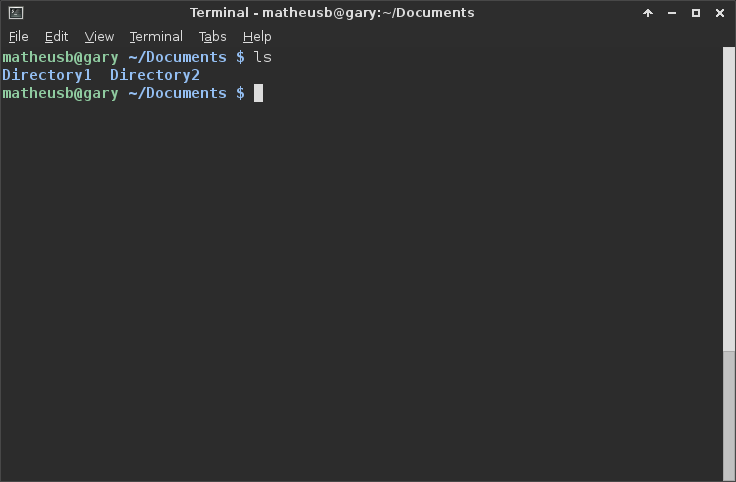
\includegraphics[scale=0.30]{ls1.png}
        \caption{Comando ls}
        \label{fig:Comando ls}
    \end{figure}
\end{frame}

\begin{frame}{Arquivos e Diretórios}{ls (list)}
  \begin{itemize}
  \item {
   O comando \textbf{ls} não mostra de fato todos os arquivos contidos na pasta atual, em sistemas Unix alguns arquivos podem ser nomeados com um ponto no início ("."), estes arquivos são chamados de arquivos ocultos. 
  }
 \end{itemize}
 \end{frame}
 
 \begin{frame}{Listando Arquivos e Diretórios}{ls (list)}
  \begin{itemize}
  \item {
   Para listar também os arquivos ocultos, utilizamos a flag (\textbf{-a}) junto com o comando ls, estas flags modificam o comportamento do comando, falaremos mais sobre isto no curso.
  }
 \end{itemize}
  \begin{figure}[h!]
        \centering
        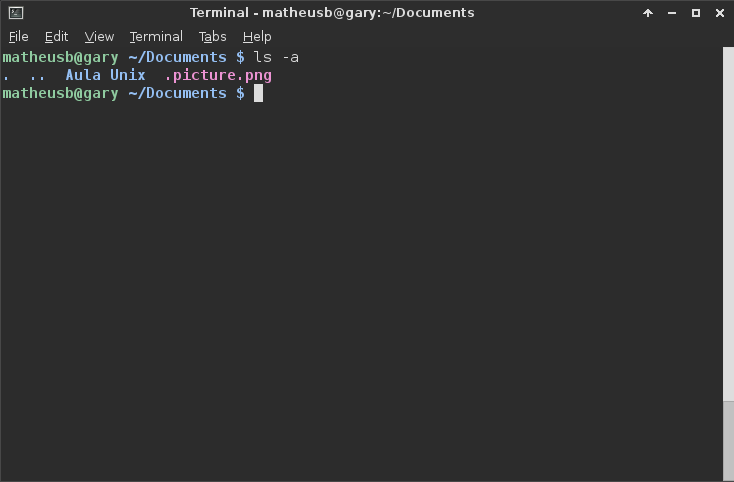
\includegraphics[scale=0.30]{ls-a.png}
        \caption{Comando ls -a}
        \label{fig:Comando ls}
    \end{figure}
\end{frame}

\subsection{touch}

\begin{frame}{touch}
  \begin{itemize}
  \item {
   O comando \textbf{touch nome.extensão} cria no seu diretório atual um arquivo chamado \textit{nome.extensão}, falaremos mais sobre extensões a frente.
  }
 \end{itemize}
   \begin{figure}[h!]
        \centering
        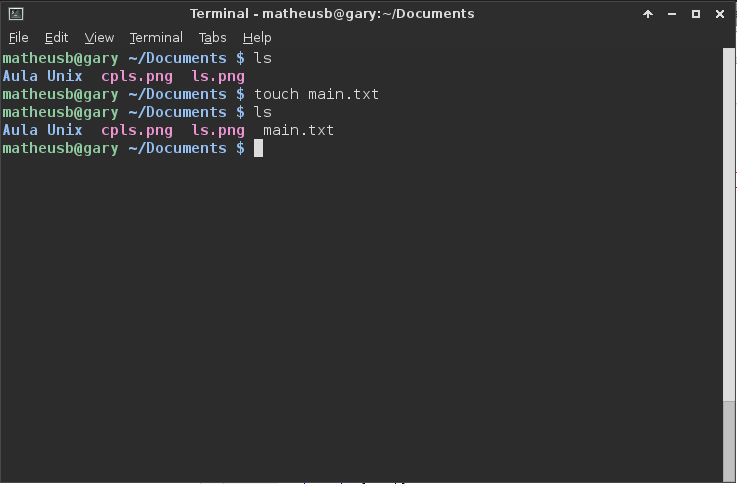
\includegraphics[scale=0.30]{touch.png}
        \caption{Comando touch}
        \label{fig:Comando touch}
    \end{figure}
\end{frame}


\subsection{mkdir (make directory)}

\begin{frame}{mkdir (make directory)}
  \begin{itemize}
  \item {
   O comando \textbf{mkdir arquivos} cria no seu diretório atual um subdiretório chamado \textit{arquivos}.
  }
 \end{itemize}
   \begin{figure}[h!]
        \centering
        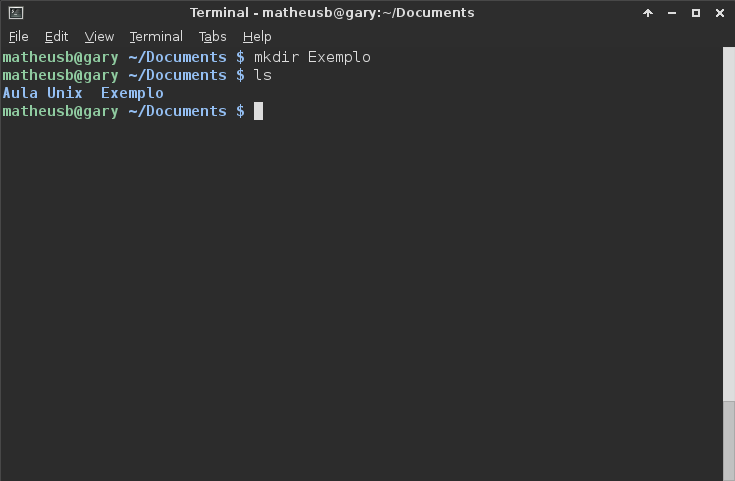
\includegraphics[scale=0.30]{mkdir.png}
        \caption{Comando mkdir}
        \label{fig:Comando mkdir}
    \end{figure}
\end{frame}

\subsection{cd (change directory)}

\begin{frame}{cd (change directory)}
  \begin{itemize}
  \item {
   O comando \textbf{cd \textit{arquivos}} modifica o diretório atual para \textit{arquivos}.
  }
 \end{itemize}
   \begin{figure}[h!]
        \centering
        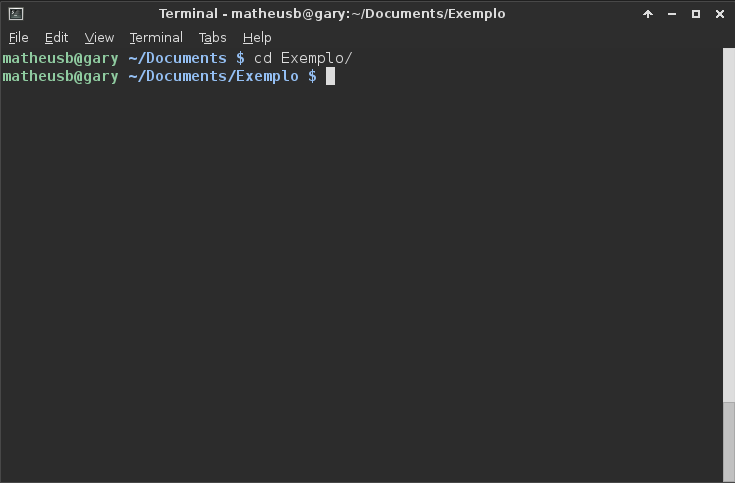
\includegraphics[scale=0.30]{cd.png}
        \caption{Comando cd}
        \label{fig:Comando cd}
    \end{figure}
\end{frame}

\subsection{pwd (print working directory)}

\begin{frame}{pwd (print working directory)}
  \begin{itemize}
  \item {
   O comando \textbf{pwd} mostra o caminho absoluto do diretório atual em rela\c{c}ão ao sistema.
  }
 \end{itemize}
   \begin{figure}[h!]
        \centering
        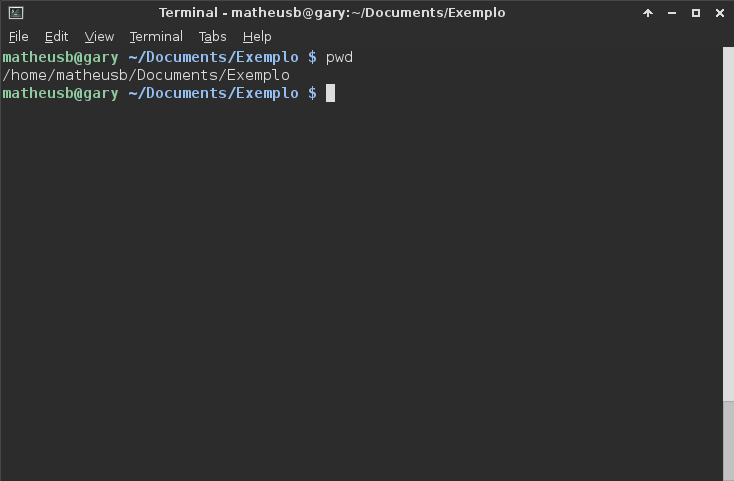
\includegraphics[scale=0.30]{pwd.png}
        \caption{Comando pwd}
        \label{fig:Comando pwd}
    \end{figure}
\end{frame}


 \begin{frame}{pwd (print working directory)}
  \begin{itemize}
  \item {
   Na imagem abaixo podemos ver o caminho absoluto do diretório \textit{Exemplo} em rela\c{c}ão ao sistema:\textbf{/home/matheusb/Documents/Exemplo}.
  }
 \end{itemize}
  \begin{figure}[h!]
        \centering
        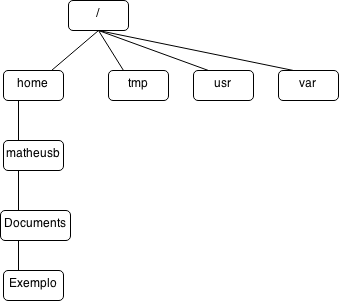
\includegraphics[scale=0.39]{unixh.png}
        \caption{Hierarquia dos diretórios}
        \label{fig:hierarquia}
    \end{figure}
\end{frame}

\section{Exercício}

\subsection{Criando diretórios}
 \begin{frame}{Comando mkdir e cd}
  \begin{itemize}
  \item {
   Utilizando o comando \textbf{mkdir} crie um diretório dentro do seu diretório atual com o nome \textit{unix}, após isso utilize o comando \textbf{cd} para navegar até o diretório criado e crie outro diretório chamado \textit{fedora}.
  }
  \item {
   Novamente, utilize o comando \textbf{cd} para navegar ao diretorio fedora, dentro do diretório fedora, utilize o comando para criar um arquivo, \textbf{touch} com a extensão \textit{.txt}.
  }
  \item {
   Utilize o comando \textbf{cd} para retornar a sua \textit{home}.
  }
 \end{itemize}
\end{frame}



\section{Um pouco mais sobre diretórios e pathnames}

\subsection{Entendendo pathnames}
 \begin{frame}{Entendendo pathnames}
  \begin{itemize}
  \item {
   Utilize o comando \textbf{ls} para listar os diretórios e arquivos contidos no diretório \textit{unix} criado no exercício, agora tente listar o que há dentro do diretório fedora desta forma: \textbf{ls fedora}. Você irá receber a seguinte mensagem: \textit{fedora: No such file or directory}.}
   \item{Isto ocorre porque não é possível utilizar um comando em um diretório que não é o atual, a não ser que você utilize o caminho completo do diretório que deseja ou utilize o comando \textbf{cd} o torne como seu diretório atual. Tente agora listar o que há dentro do diretório fedora desta forma: \textbf{ls unix/fedora}.}
 \end{itemize}
\end{frame}

% Placing a * after \section means it will not show in the
% outline or table of contents.
\section*{Sumário dos comandos}

\begin{frame}{Sumário dos comandos}
 \begin{center}
 \begin{tabular}{||c | c||} 
 \hline
 Comando & Descri\c{c}ão\\ [0.5ex] 
 \hline\hline
 ls & Lista os diretórios e arquivos contidos no diretório atual\\ 
 \hline
 touch & Cria um arquivo com o nome e a extensão desejados\\
 \hline
 mkdir & Cria um diretório dentro do diretório atual\\
 \hline
 cd & Modifica o diretório atual para o desejado\\
 \hline
 pwd & Lista o caminho absotulo do diretório atual  \\
 \hline
\end{tabular}
\end{center}
\end{frame}

\end{document}


